% Chapter 2: Market Overview & Definition
\chapter{Panorama del Mercado Minero}

\section{Definición y Alcance}

\begin{calloutbox}[Definición del Mercado]
El presente análisis abarca el mercado de \textbf{consultoría de ingeniería minera}: servicios de estudios de factibilidad, planificación minera, diseño de plantas de procesamiento, optimización operacional, gestión de proyectos (EPCM) y asesoría ESG para operaciones mineras. El alcance geográfico cubre los cinco países de operación del cliente: \highlight{Chile, Brasil, Perú, Estados Unidos y Rusia}. Horizonte temporal: 2026--2031 (5 años).
\end{calloutbox}

\subsection{Ecosistema de la Industria}

La cadena de valor de la consultoría de ingeniería minera opera en la intersección entre los \textbf{operadores mineros} (demanda) y los \textbf{proveedores de tecnología/equipos} (oferta complementaria). El consultor de ingeniería actúa como integrador de conocimiento técnico en todas las fases del ciclo de vida minero:

\begin{enumerate}
    \item \textbf{Exploración y Evaluación:} Estudios geológicos, estimación de recursos (NI 43-101, JORC).
    \item \textbf{Pre-factibilidad y Factibilidad:} Diseño conceptual, análisis económico, DFS/PFS.
    \item \textbf{Ingeniería y Construcción:} EPCM, ingeniería de detalle, gestión de construcción.
    \item \textbf{Operación y Optimización:} Optimización de procesos, eficiencia energética, automatización.
    \item \textbf{Cierre y Remediación:} Planes de cierre, restauración ambiental, pasivos.
\end{enumerate}

\section{Tamaño y Crecimiento del Mercado}

\begin{figure}[htbp]
\centering
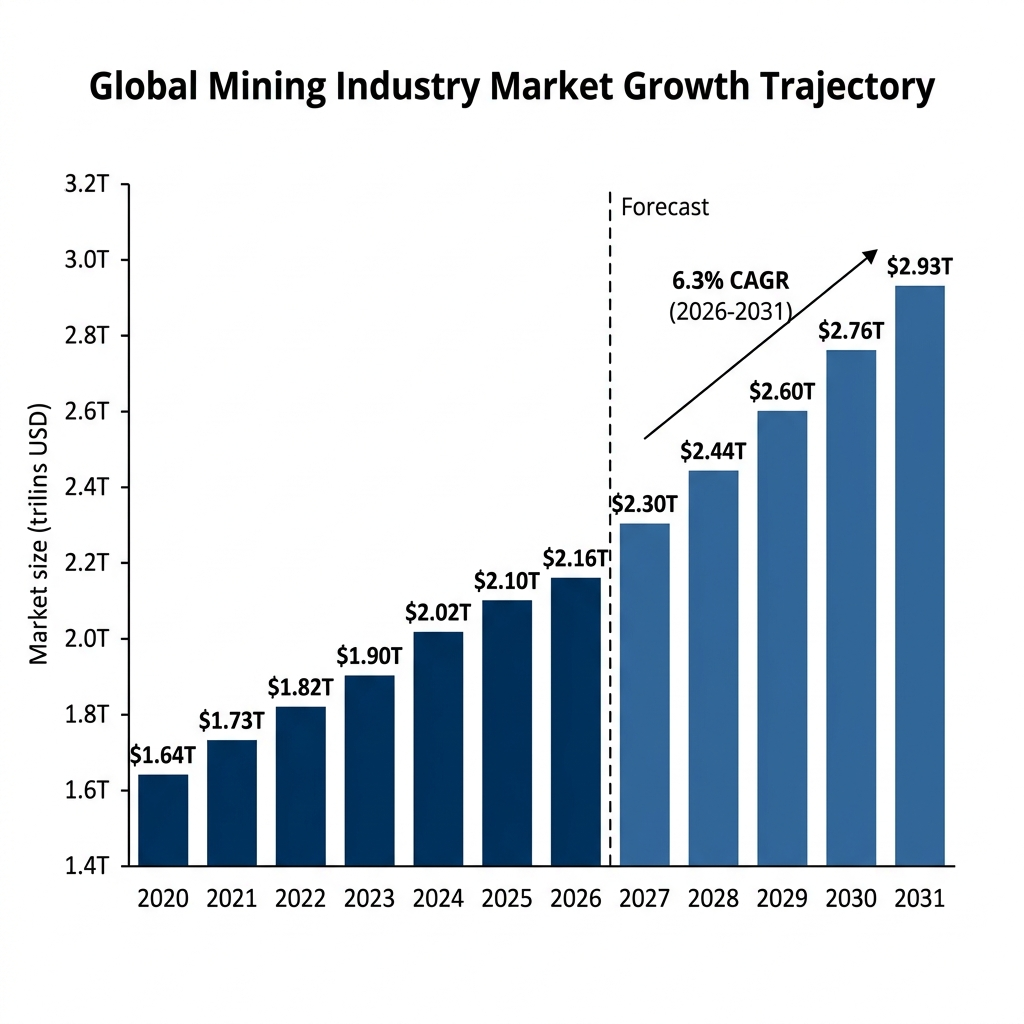
\includegraphics[width=0.92\textwidth]{../figures/01_market_growth_trajectory.png}
\caption{Trayectoria de Crecimiento del Mercado Minero Global (2020--2031). Fuente: Research and Markets \cite{researchandmarkets2026}, análisis propio.}
\label{fig:market_growth}
\end{figure}

El mercado minero global alcanzó \marketsize{2.16 trillones} en 2026 \cite{researchandmarkets2026}, con una proyección a \marketsize{2.93 trillones} para 2031 (CAGR \growthrate{6.3}). El segmento específico de consultoría de ingeniería minera fue valorado en \marketsize{12.8 mil millones} en 2025, con proyección a \marketsize{22.6 mil millones} para 2034 (CAGR \growthrate{6.5}) \cite{dataintelo2025}.

\subsection{TAM / SAM / SOM}

\begin{figure}[htbp]
\centering
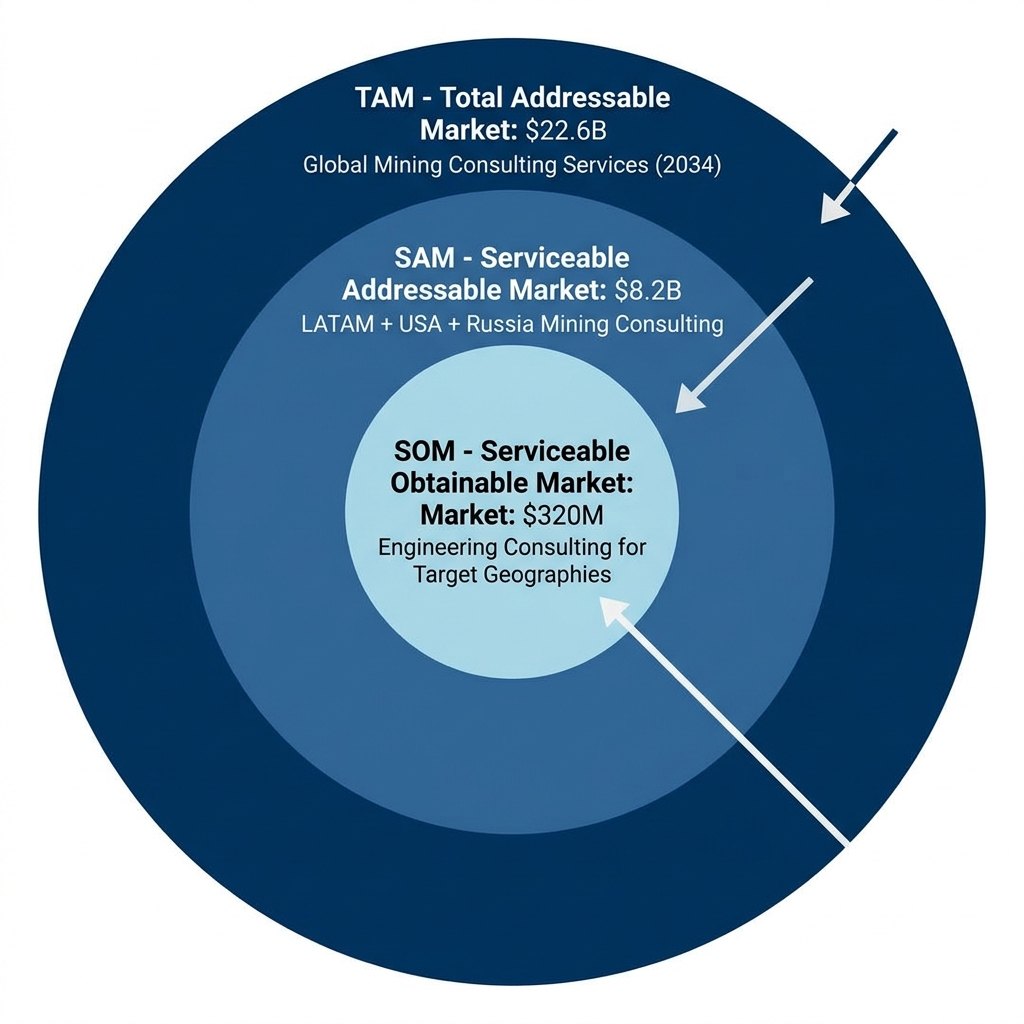
\includegraphics[width=0.75\textwidth]{../figures/02_tam_sam_som.png}
\caption{Desglose TAM/SAM/SOM del Mercado de Consultoría de Ingeniería Minera. Fuente: Dataintelo \cite{dataintelo2025}, análisis propio.}
\label{fig:tam_sam_som}
\end{figure}

\begin{table}[htbp]
\centering
\caption{Dimensionamiento de Mercado: TAM / SAM / SOM}
\begin{tabular}{@{}lrrp{5.5cm}@{}}
\toprule
\textbf{Nivel} & \textbf{Valor (USD)} & \textbf{CAGR} & \textbf{Definición} \\
\midrule
TAM & \$22.6B (2034) & 6.5\% & Mercado global de consultoría minera \cite{dataintelo2025} \\
\rowcolor{tablealt} SAM & \$8.2B & 7.1\% & Consultoría en Chile, Brasil, Perú, USA, Rusia \\
SOM & \$320M & 8.5\% & Ingeniería especializada en geografías objetivo \\
\bottomrule
\end{tabular}
\label{tab:tam_sam_som}
\end{table}

\subsection{Análisis Regional de Inversión Minera}

\begin{figure}[htbp]
\centering
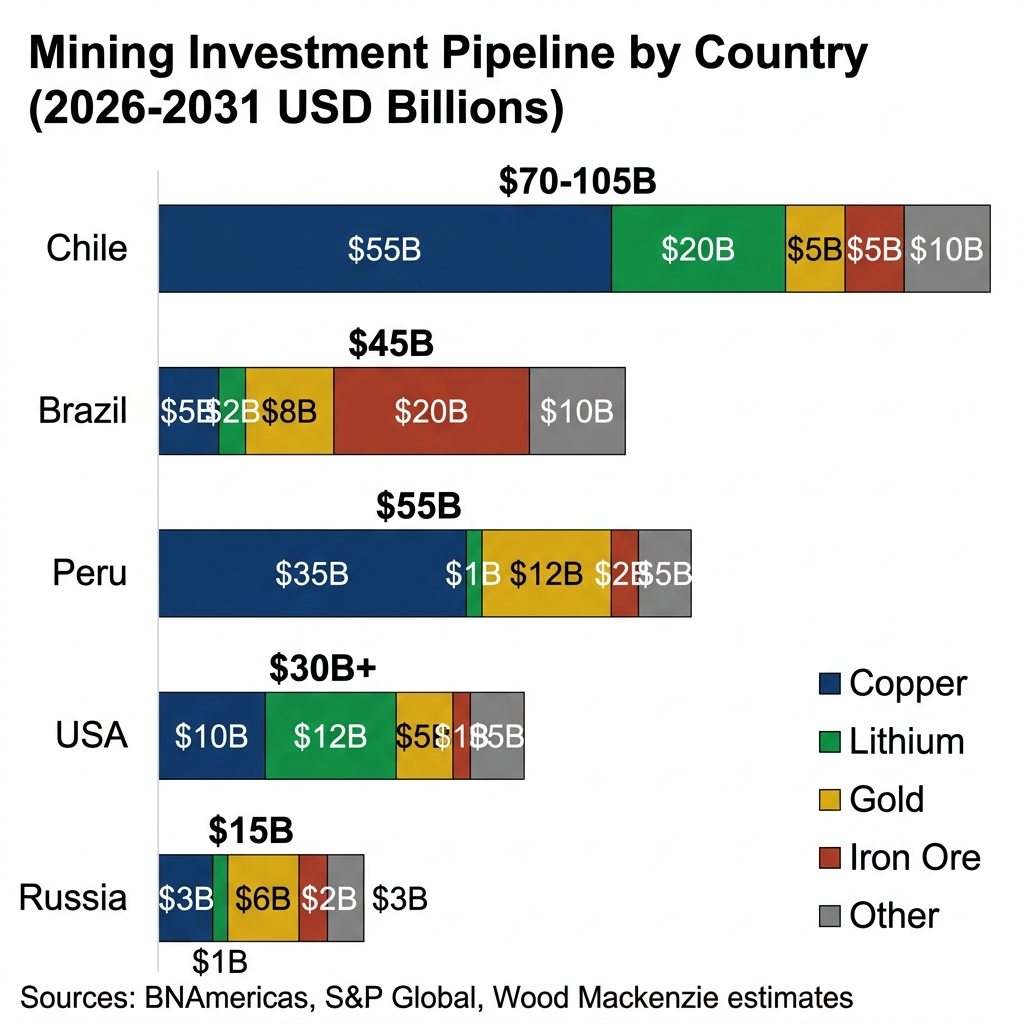
\includegraphics[width=0.92\textwidth]{../figures/06_regional_capex.png}
\caption{Pipeline de Inversión Minera por País (2026--2031, USD Miles de Millones). Fuentes: BNAmericas \cite{bnamericas2026}, S\&P Global \cite{spglobal2026}, Wood Mackenzie \cite{woodmac2026}.}
\label{fig:regional_capex}
\end{figure}

\begin{table}[htbp]
\centering
\caption{Inversión Minera por País: Pipeline y Proyecciones}
\begin{tabular}{@{}lrrrr@{}}
\toprule
\textbf{País} & \textbf{Pipeline} & \textbf{CAPEX 2026} & \textbf{Mineral Core} & \textbf{Riesgo} \\
\midrule
Chile & \$70--105B & \$8.5B & Cobre, Litio & \risklow{} \\
\rowcolor{tablealt} Perú & \$55B & \$6.3B & Cobre, Oro & \riskmedium{} \\
Brasil & \$45B & \$5.2B & Hierro, Litio & \risklow{} \\
\rowcolor{tablealt} USA & \$30B+ & \$4.8B & Litio, Cu, REE & \risklow{} \\
Rusia & \$15B & \$3.5B & Oro, Cobre & \riskhigh{} \\
\bottomrule
\end{tabular}
\label{tab:regional_capex}
\end{table}

\paragraph{Chile.} El pipeline cuprífero de USD 70--105B hasta 2034 es el mayor del mundo \cite{cochilco2026}. El 81\% corresponde a proyectos brownfield (expansiones, optimizaciones, continuidades operacionales). Factores limitantes: leyes de mineral decrecientes, escasez hídrica y procesos de permisos extensos. Reformas regulatorias recientes buscan simplificar el licenciamiento.

\paragraph{Perú.} Mantiene un portafolio de proyectos mineros valorado en más de USD 55B, con inversión privada en trayectoria ascendente hacia USD 6.3B a fin de 2026 \cite{andina2026peru}. El avance de proyectos greenfield está restaurando la confianza de los inversionistas.

\paragraph{Brasil.} Potencia en hierro (17.5\% de la oferta global), con creciente prominencia en litio y tierras raras. El 75\% del tráfico ferroviario brasileño está dedicado a la minería, con nuevos proyectos de infraestructura logística en desarrollo \cite{bnamericas2026}.

\paragraph{Estados Unidos.} Política de ``America First'' en minerales críticos: >USD 30B movilizados en préstamos, equity y apoyo federal. Instalaciones militares albergan plantas de procesamiento de tierras raras, litio y grafito (acuerdos con REalloys, Titan Mining, ioneer, EnergyX en 2026).

\paragraph{Rusia.} Polyus alcanzó inversiones récord de USD 2.2B en 2025 (proyección similar para 2026), centrado en el depósito Sukhoi Log (estimado en USD 6B, operación plena 2029) \cite{polyus2025}. Seligdar reportó crecimiento de ingresos del 49\% en oro \cite{seligdar2025}. Nornickel proyecta +10\% en producción de concentrado de cobre para 2026. \textbf{Riesgo:} sanciones occidentales elevan costos y complican acceso a capital y tecnología.

\begin{riskbox}[Efecto Seligdar/Rusia — Alerta Crítica para REDCO]
Los contratos rusos (Seligdar/Polyus/AtlasMining) inflan el POM pero \textbf{no convierten a caja} (Real $\approx$ 0, EDP = 0). El POM bruto \textbf{sobreestima} el ingreso. El modelo de flujo de caja (archivo 05) incluye un toggle ``Efecto Seligdar\_Rusia'' — este es el nodo de decisión/escenario más importante del proyecto. Recomendación: operar con flujo ajustado como escenario base.
\end{riskbox}
